\documentclass[a4paper,11pt]{article}
\usepackage{amsmath, amsthm, amssymb, atbegshi, booktabs, hyperref, listings, newpxmath, sectsty, subcaption, tikz, wrapfig, xcolor, xfrac}
%\usepackage[bitstream-charter]{mathdesign}
%\usepackage[T1]{fontenc}
\usepackage{ebgaramond}
\usepackage[semibold]{sourcesanspro}
\usepackage[inline]{enumitem}
\usepackage[margin=1in]{geometry}
\hypersetup{colorlinks = true, allcolors = othelloGreen}

\usetikzlibrary{shapes.misc}
\usetikzlibrary{calc}

\pgfdeclarelayer{bg}
\pgfsetlayers{bg, main}

\allsectionsfont{\sffamily}

% Custom Captions

\DeclareCaptionFormat{custom}
{%
	{\sffamily\footnotesize\textbf{#1#2}{ #3}}
}
\captionsetup{format=custom}

\allowdisplaybreaks

%\AtBeginShipout{\ifnum\value{page}=7\pagecolor{gray!20}\fi}

\title{\sffamily\LARGE\textbf{Coachello Demo Script}\\\Large A quick demo of Machine Coaching}
\author{\sffamily V. Markos}
\date{\sffamily\today}

\renewenvironment{abstract}
{\small
	\begin{center}
		\sffamily\bfseries \abstractname\vspace{-.5em}\vspace{0pt}
	\end{center}
	\list{}{%
		\setlength{\leftmargin}{35mm}
		\setlength{\rightmargin}{\leftmargin}%
	}%
	\item\relax}
{\endlist}

% Custom colors

\definecolor{c1}{HTML}{ac0000}
\definecolor{c2}{HTML}{0000ac}
\definecolor{c3}{HTML}{00ac00}

\definecolor{othelloBlack}{HTML}{051005}
\definecolor{othelloGreen}{HTML}{4f8a8b}

% Number sets

\newcommand{\Co}{\mathbb{C}}
\newcommand{\R}{\mathbb{R}}
\newcommand{\Q}{\mathbb{Q}}
\newcommand{\Z}{\mathbb{Z}}
\newcommand{\N}{\mathbb{N}}

% QM notation

\newcommand{\bra}[1]{{\left\langle{#1}\right|}} 
\newcommand{\ket}[1]{{\left|{#1}\right\rangle}} 
\newcommand{\abs}[1]{{\left|{#1}\right|}}
\newcommand{\ip}[2]{{\left.\left\langle{#1}\right|{#2}\right\rangle}}
\newcommand{\ep}[2]{{\left|\,{#1}\left\rangle\vphantom{#1}\vphantom{#2}\right\langle{#2}\,\right|}}
\newcommand{\dCol}[2]{{\left[\begin{array}{c}
			{#1} \\[1.4ex]
			{#2}
		\end{array}\right]}}
\newcommand{\dRow}[2]{{\left[{#1}\quad{#2}\right]}}
\newcommand{\qCol}[4]{\qn{\begin{array}{c}
			{#1} \\ {#2} \\ {#3} \\ {#4}
\end{array}}}
\newcommand{\qmatr}[4]{{\left[\begin{array}{cc}
			{#1} & {#2}\\[1.4ex]
			{#3} & {#4}
		\end{array}\right]}}
\newcommand{\pn}[1]{\left({#1}\right)}
\newcommand{\qn}[1]{\left[{#1}\right]}

% Operators

\newcommand{\unot}{U_{\sqrt{\rm NOT}}}
\newcommand{\id}{I}
\newcommand{\noact}{\qmatr{1}{0}{0}{1}}
\newcommand{\had}[1][\frac{1}{\sqrt{2}}]{#1\qmatr{1}{1}{1}{-1}}
\newcommand{\notop}{\qmatr{0}{1}{1}{0}}
\newcommand{\zeros}{\mathbb{O}}
\newcommand{\zerop}{\qmatr{0}{0}{0}{0}}
\newcommand{\cnot}{\qn{\begin{array}{cccc}
	1 & 0 & 0 & 0 \\
	0 & 1 & 0 & 0 \\
	0 & 0 & 0 & 1 \\
	0 & 0 & 1 & 0
\end{array}}}
\newcommand{\idfour}{\qn{\begin{array}{cccc}
			1 & 0 & 0 & 0 \\
			0 & 1 & 0 & 0 \\
			0 & 0 & 1 & 0 \\
			0 & 0 & 0 & 1
\end{array}}}

% Python listing

\DeclareFixedFont{\ttb}{T1}{txtt}{bx}{n}{8} % for bold
\DeclareFixedFont{\ttm}{T1}{txtt}{m}{n}{8}  % for normal

\newcommand\pythonstyle{\lstset{
		language=Python,
		basicstyle=\ttm\linespread{0.4},
		morekeywords={self, if, for, in, import, as, from},              % Add keywords here
		keywordstyle=\ttb\color{c1},
		emph={__name__, def, lambda, matplotlib, pyplot, plt, numpy, np, scipy, integrate, special, jv, solve_ivp},          % Custom highlighting
		emphstyle=\ttb\color{c2},    % Custom highlighting style
		stringstyle=\color{c3},
		frame=tb,                         % Any extra options here
		showstringspaces=false
}}

% Python environment
\lstnewenvironment{python}[1][]
{
	\pythonstyle
	\lstset{#1}
}
{}

% Python for external files
\newcommand\pythonexternal[2][]{{
		\pythonstyle
		\lstinputlisting[#1]{#2}}}

% Python for inline
\newcommand\pythoninline[1]{{\pythonstyle\lstinline!#1!}}

% End of Python listing

\let\Re\relax
\DeclareMathOperator{\Re}{Re}

\theoremstyle{definition}

\newtheorem{exercise}{Exercise}[section]
\newtheorem{lemma}{Lemma}[section]

\theoremstyle{remark}
\newtheorem*{comment}{Comment}

%\setcounter{section}{3}

\numberwithin{equation}{section}

\begin{document}
	\maketitle
	
	\begin{abstract}
		In this quick walk-through we demonstrate a script for a quick demo of Machine Coaching through the Coachello GUI. All mentioned saved games might be found in \texttt{../games} directory.
	\end{abstract}

	\section{Script}\label{sec:Script}
	%
	We present the script into three parts, one per each reviewed game.
	%
	%
	%
	\subsection{First Round: Play on the Sides}\label{subsec:First Round}
	%
	\begin{enumerate}
		\item Open the online GUI, available at: \href{https://vmarkos.github.io/coachello/}{\texttt{https://vmarkos.github.io/coachello/}}.
		\item Press the ``Audit'' button and load the game found in:  \href{../games/hp_47_17_1679552346213.json}{\texttt{hp\textunderscore 47\textunderscore 17\textunderscore 1679552346213.json}}.
	\end{enumerate}
	\begin{minipage}[c]{0.6\textwidth}
		\begin{enumerate}
			\setcounter{enumi}{2}
			\item Press the white dot (intermediate state) on the third row, right before white's move C5.			
			\item At this point, we would like the agent to have played to the available side cell at A4, so the next step is to press the ``Offer advice'' button.
			\item Offer the advice shown in Figure~\ref{fig:101}, by double-clicking on D8 and making a single click on the cell below it.
			\item Click the ``Done'' button on the bottom right of the screen to return to the game screen.
			\item Press the white download button to (demonstrate how to) download the coached policy, as shown in Figure~\ref{fig:102}.
		\end{enumerate}
	\end{minipage}\hfill
	%
	\begin{minipage}[c]{0.35\textwidth}
		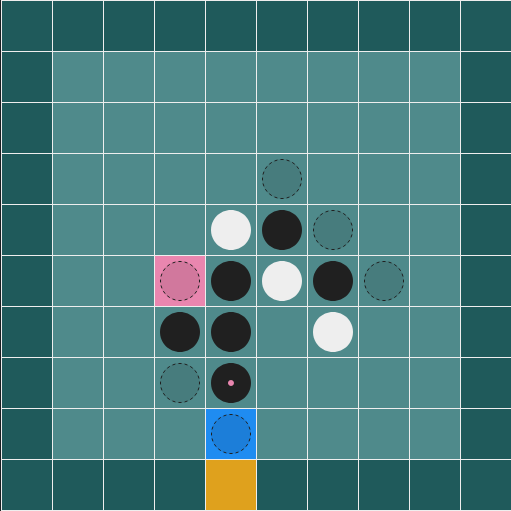
\includegraphics[width = \textwidth]{../assets/advice_001.png}
		\captionof{figure}{The first piece of advice.}
		\label{fig:101}
	\end{minipage}

	\begin{figure}[!htb]
		\centering
		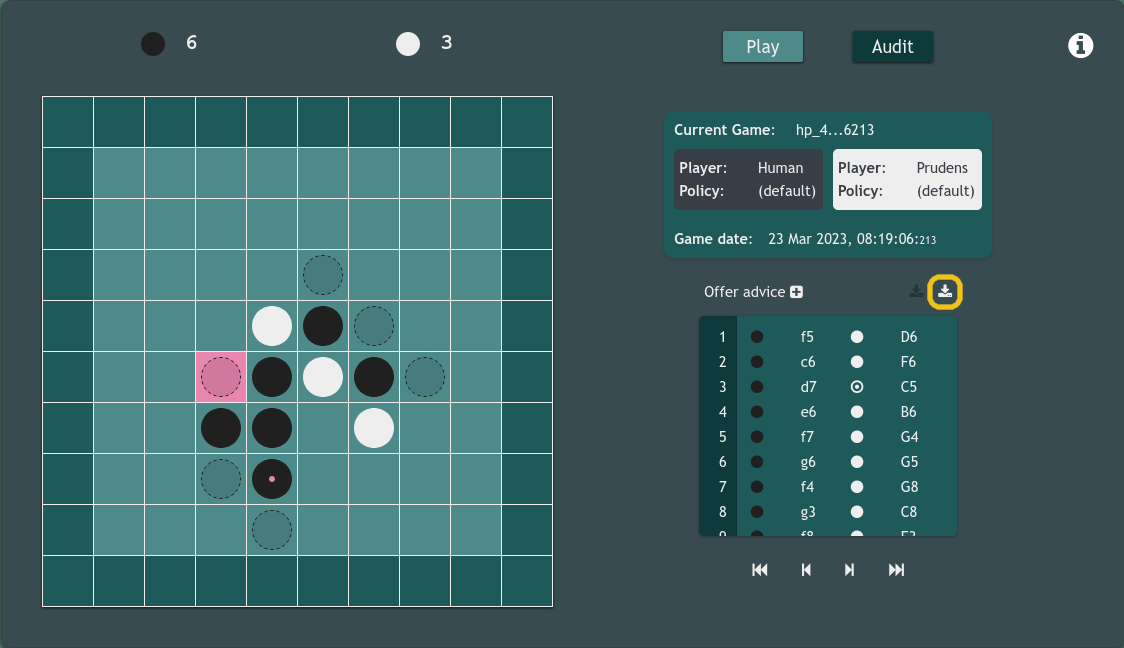
\includegraphics[width = 0.8\textwidth]{../assets/download_coached_policy.png}
		\caption{Downloading the first version of our coached policy (by pressing the button marked by a yellow rounded rectangle).}
		\label{fig:102}
	\end{figure}
	%
	%
	%
	\subsection{Second Round: Don't Play Next to Corners}\label{subsec:Round Two}
	%
	\begin{enumerate}
		\item Load the following game in audit mode: \href{../games/hp_50_14_1679553207662.json}{\texttt{hp\textunderscore 50\textunderscore 14\textunderscore 1679553207662.json}}.
		\item At first, go to the intermediate state before H5 (5\textsuperscript{th} row, white dot) to showcase how the agent, when it has more than two suggested moves to play, chooses at random --- see Figure~\ref{fig:201a}.
		\item Go to the intermediate state before white's move H7 (6\textsuperscript{th} row, white dot) --- Figure~\ref{fig:201b}.
		\item There you shall now see that there is a blue border around the played move. Hover over that cell to show the explanation's body, which corresponds to (a rotated version of) the advice we provided before\footnote{Depending on the audience and time available, one could present other white moves to some side of the board such as G8 (line 16) which is also a corner move.}.
		\item At this point, we would like to offer some advice regarding avoiding to play next to corners. To do so, press again the ``Offer advice'' button and provide the piece of advice shown on Figure~\ref{fig:201c}. After providing the first piece of advice, press the ``Advise'' button and not the ``Done'' button, since we want to provide a second pattern\footnote{At this point we could probably make a point about how using the auxiliary border cells corresponds, essentially, to using Cartesian coordinates over the board.}.
		\item Then, provide the second piece of advice, as shown in Figure~\ref{fig:201d}.
		\item Once done, press the ``Done'' button and download again the coached policy\footnote{As with the first game, we are downloading each coached policy just to showcase the corresponding functionality. In practice, each version of the coached policy is embedded into each save game file.}.
	\end{enumerate}

	\begin{figure}[!htb]
		\centering
		\begin{subfigure}[t]{0.48\textwidth}
			\centering
			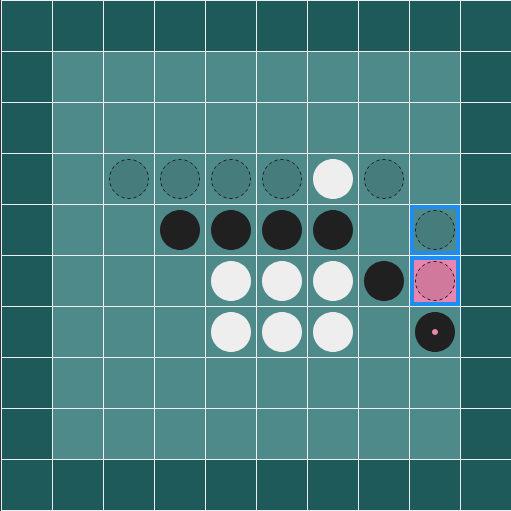
\includegraphics[width = \textwidth]{../assets/coaching_success_001.png}
			\caption{When having to choose between more than two ``good'' moves, the machine chooses at random among them.}
			\label{fig:201a}
		\end{subfigure}\hfill
		\begin{subfigure}[t]{0.48\textwidth}
			\centering
			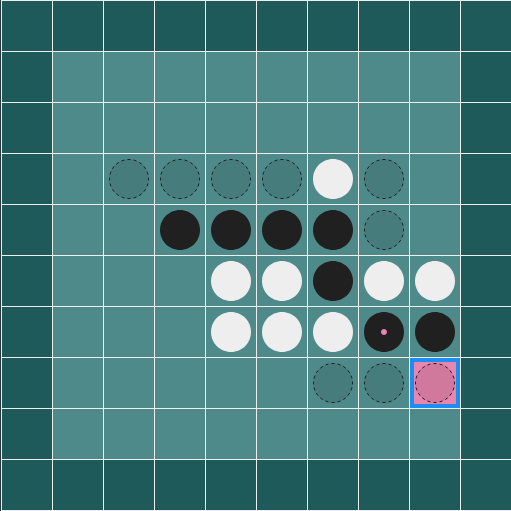
\includegraphics[width = \textwidth]{../assets/coaching_failure_001.png}
			\caption{The machine plays according to our previous advice, but, now, we would like to avoid playing to that side cell.}
			\label{fig:201b}
		\end{subfigure}\\
		\vspace{2\topsep}
		\begin{subfigure}[t]{0.48\textwidth}
			\centering
			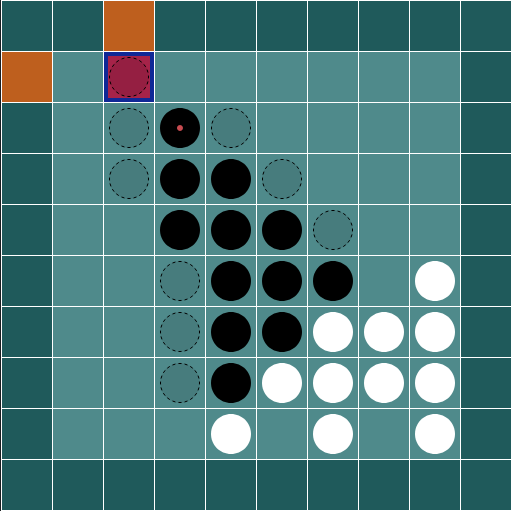
\includegraphics[width = \textwidth]{../assets/advice_002.png}
			\caption{Instructing Prudens not to play next to corner cells (sides).}
			\label{fig:201c}
		\end{subfigure}\hfill
		\begin{subfigure}[t]{0.48\textwidth}
			\centering
			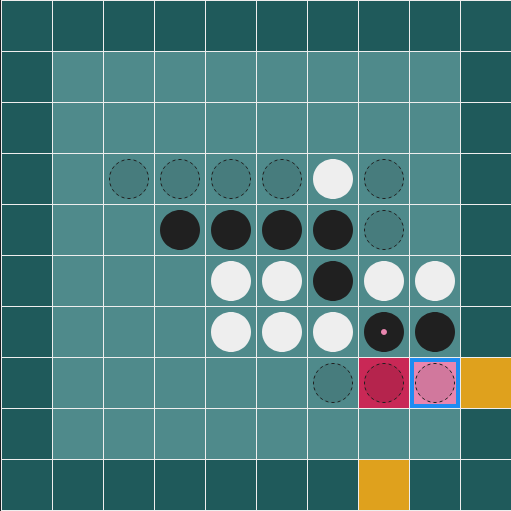
\includegraphics[width = \textwidth]{../assets/advice_003.png}
			\caption{Instructing Prudens not to play next to corner cells (diagonals).}
			\label{fig:201d}
		\end{subfigure}
		\caption{The next two pieces of advice that intend to prohibit the machine from playing next to corners.}
		\label{fig:201}
	\end{figure}
	%
	%
	%
	\subsection{Third Round: Showcasing Overall Behavior}\label{subsec:Third Round}
	%
	\begin{minipage}{0.60\textwidth}
		\begin{enumerate}
			\item Load the following game in audit mode: \href{../games/hp_10_54_1679554654733.json}{\texttt{hp\textunderscore 10\textunderscore 54\textunderscore 1679554654733.json}}.
			\item Move to the intermediate state (white dot) before whites move to F4 (2\textsuperscript{nd} row). There, we can observe how the machine avoid to play to G7 (you can hover over G7 to see the explanation).
			\item Then, click on the intermediate state before the white's move to H5 (6\textsuperscript{th} row, white dot). There we can observe how the machine avoids to play at several ``bad'' positions while it chooses at random among the suggested ones --- see Figure~\ref{fig:301}.
			\item Then, you may also click on the intermediate state before white's move to B2 (26\textsuperscript{th} row) to demonstrate a case where all remaining moves are not suggested. In that case, as discussed, the machine plays at random.
		\end{enumerate}
	\end{minipage}\hfill
	\begin{minipage}{0.35\textwidth}
		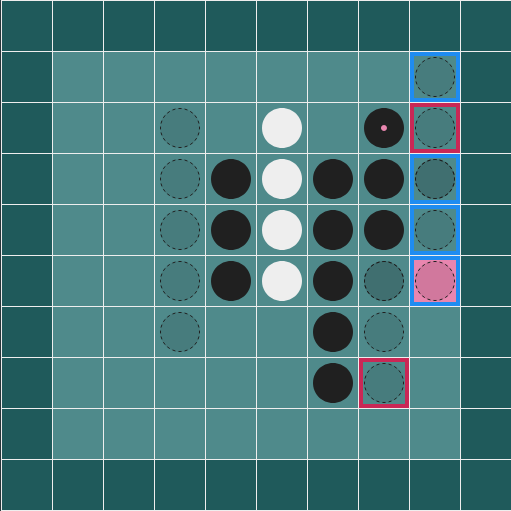
\includegraphics[width = \textwidth]{../assets/coaching_success_002.png}
		\captionof{figure}{Choosing at random among any ``good'' moves while avoiding ``bad'' ones.}
		\label{fig:301}
	\end{minipage}
\end{document}